%---------------------------------------------------------------------------------------------------
%		network.tex
%
%	This is file contains the network measurements.
%
%	Author: Andrea Meneghinello
% Version: 0.1
%	Table of changes:
%		21/03/2016 -> document definition
%---------------------------------------------------------------------------------------------------
\section{Network benchmark}
\label{sec:measurements-network}
By means of Iperf benchmark tool we want to measure how the different virtualization environments
can exploit the available bandwidth and the network latency. In order to have a basis for comparison 
we initially have executed the tests on the two native machines and then in the following environments:

\begin{enumerate}
	\item{two Docker containers placed in different physical machines;}
	\item{two \ac{kvm} \ac{vm}s placed in different physical machines.}
\end{enumerate}

As previously said in the chapter introduction, the two physical machines are linked together in a \acs{lan}
through a Netgear M7300 series Gigabit switch by means of optical fibre cables.

\subsection{Iperf benchmark}
\label{sec:measurements-network-nuttcp}
Iperf is a network performance measurement tool intended for use by network and system managers. Its
most basic usage is to determine the raw \acs{tcp} (or \acs{udp}) network layer throughput by transferring
memory buffers from a source system across an interconnecting network to a destination system, either
transferring data for a specified time interval, or alternatively transferring a specified number of bytes.
In addition to reporting the achieved network throughput in Mbps, iperf also provides additional useful
information related to the data transfer such as user, system, and wall-clock time, transmitter and receiver
\acs{cpu} utilization, and loss percentage (for \acs{udp} transfers).

Iperf allows network managers to set various parameters that can be used for testing, optimizing
or tuning a network. Iperf has a \keyword{client} and \keyword{server} functionality, and can
measure the throughput between the two ends, either unidirectionally or bi-directionally. Typical Iperf output
contains a time-stamped report of the amount of data transferred and the throughput measured.

\subsection{Configuration}
\label{sec:measurements-network-configuration}
To measure both the network bandwidth and latency we have used similar network configurations. When we have
tested the network bandwidth, we do not have forced the tool with any parameter, so it was able to adjust network
parameters, like network windows, automatically.

Instead, when we had measured the network latency we have configured the tool so that it was able to send
a packet and wait for the server response before it could send another request. Thus only one transaction is
in flight at a time. 

\subsection{Results}
\label{sec:measurements-network-result}
After executing the tests in all the environments we collected the results that are shown in Table
\ref{tbl:measurements-network-result-bandwidth} in the matter of the available network bandwidth, and
in Table \ref{tbl:measurements-network-result-latency} for those about the network latency.

\begin{center}
	\begin{tabular}{| l | c | r | r | r | r |}
		\hline
		\multicolumn{6}{| c |}{\textbf{Network throughput}}                                                                  \\ \hline
		\multicolumn{2}{| c |}{}                        &          \multicolumn{4}{c |}{\textit{Throughput (MB/s)}}          \\ \hline
		\textit{Env.}              & \textit{Direction} & \textit{Min}  & \textit{Max}  & \textit{Avg}  & \textit{Std. Dev.} \\ \hline
		\multirow{2}{*}{Native}    & C -> S             & $9\,409.8646$ & $9\,415.2581$ & $9\,414.6153$ & $0.6711$           \\ \cline{2-6}
		                           & S -> C             & $9\,410.3983$ & $9\,415.2769$ & $9\,414.6119$ & $0.6065$           \\ \hline
		\multirow{2}{*}{Docker}    & C -> S             & $9\,391.9720$ & $9\,394.8341$ & $9\,393.4361$ & $0.8175$           \\ \cline{2-6}
		                           & S -> C             & $9\,389.4003$ & $9\,391.3858$ & $9\,390.3264$ & $0.5636$           \\ \hline
		\multirow{2}{*}{\acs{kvm}} & C -> S             & $9\,356.8689$ & $9\,358.8478$ & $9\,357.8673$ & $0.5469$           \\ \cline{2-6}
		                           & S -> C             & $9\,353.4524$ & $9\,355.3841$ & $9\,354.4433$ & $0.5720$           \\ \hline
	\end{tabular}
	\captionof{table}{Network available bandwidth.}
	\label{tbl:measurements-network-result-bandwidth}
\end{center}

From the chart, illustrated in Figure \ref{img:measurements-network-results-bandwidth}, we can observe
that in matter of network bandwidth there are not substantial differences, given that all the
virtualization environments are able to get close to the theoretical limit of 9.4 Gb/s\footnote{Limit
forced by the configuration of the \acs{tcp} network protocol.}. The pattern is maintained in both
directions ()client to server one and viceversa). This leads us to affirm that the virtualization
layer does not compromise the available bandwidth in both the virtualization environments.

\begin{figure}
	\centering{}
	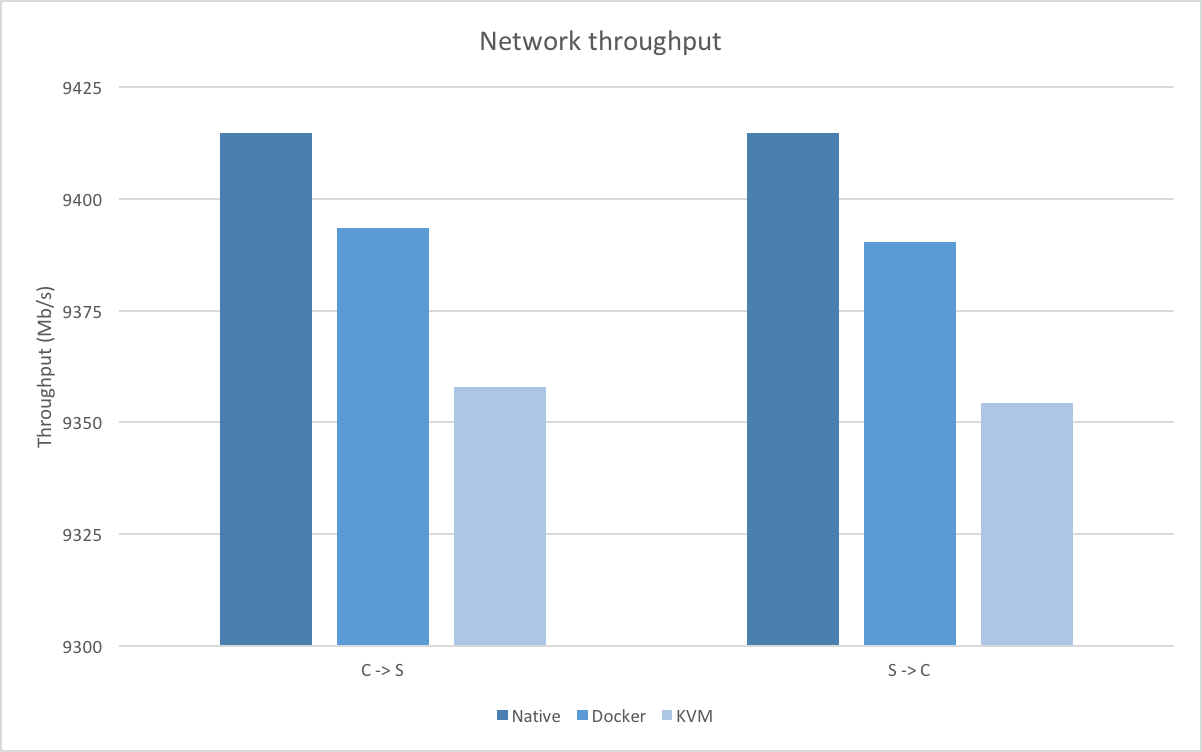
\includegraphics[width=0.8\textwidth]{chapters/measurements/images/network-throughput.png}
	\caption[Network - avaialable bandwidth]{Network available bandwidth measured.}
	\label{img:measurements-network-results-bandwidth}
\end{figure}

With respect to the network delay we have found that the \acs{os}-level virtualization, provided by 
Docker, is the one that creates the greatest delay (as Figure
\ref{img:measurements-network-results-latency} shows); it is higher, even if just a little, than the one
provided by the hardware-level virtualization which is twice that of native execution.

\begin{center}
	\begin{tabular}{| l | r | r | r | r |}
		\hline
		\multicolumn{5}{| c |}{\textbf{Network Latency}}                                \\ \hline
		&         \multicolumn{4}{c |}{\textit{Latency ($\mu$s)}}         \\ \hline
		\textit{Env.} & \textit{Min} & \textit{Max} & \textit{Avg} & \textit{Std. Dev.} \\ \hline
		Native        & $37.2296$    & $41.9557$    & $39.4489$    & $1.5114$           \\ \hline
		Docker        & $73.0843$    & $79.8891$    & $76.2959$    & $1.8605$           \\ \hline
		\acs{kvm}     & $69.0498$    & $74.9104$    & $71.8517$    & $1.4772$           \\ \hline
	\end{tabular}
	\captionof{table}{Network latency resume.}
	\label{tbl:measurements-network-result-latency}
\end{center}

\begin{figure}
	\centering{}
	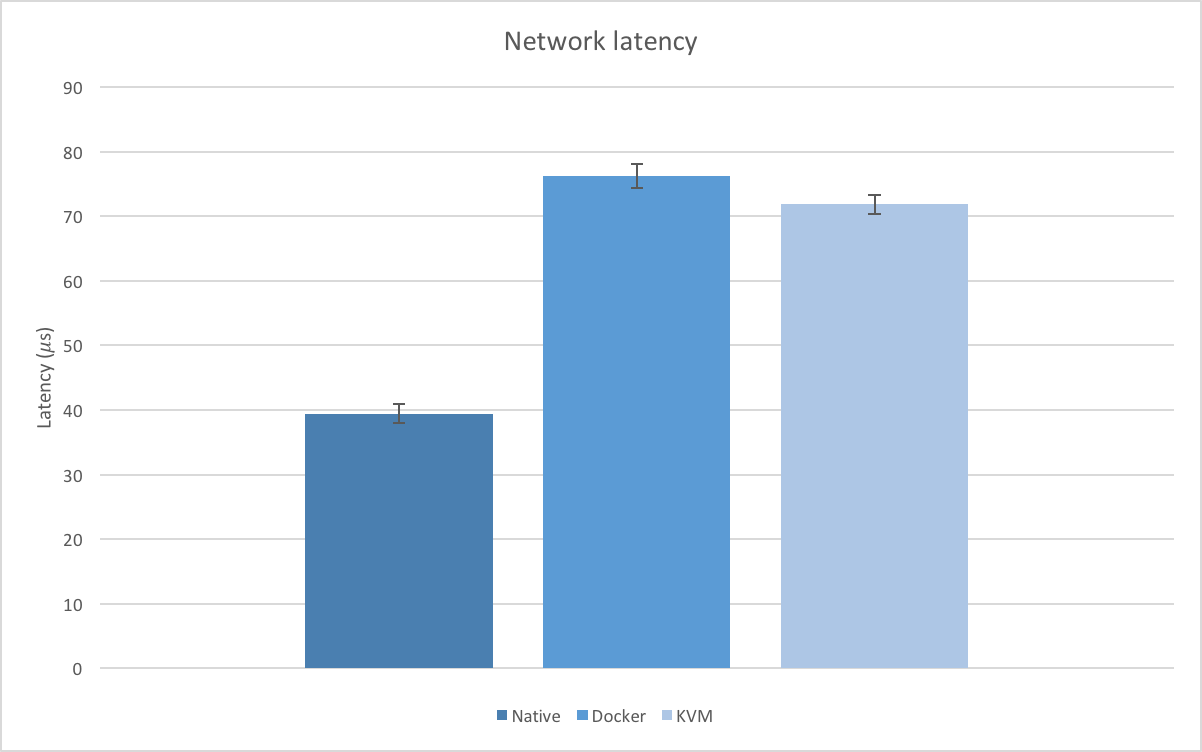
\includegraphics[width=0.8\textwidth]{chapters/measurements/images/network-latency.png}
	\caption[Network - latency measured]{Network latency measured.}
	\label{img:measurements-network-results-latency}
\end{figure}

To investigate the causes that generate this lack in performance we have analysed the stacks that divide
both the \acs{os}-level virtualization and the hardware-level virtualization from the physical world (the
different stacks are illustrated in Figure \ref{img:measurements-network-result-stacks}). Reading also
the official Docker documentation we have found that during the Docker daemon installation, on the system,
a network bridge (named ``Docker$0$'') is created. Later this bridge is linked to one of the available
\ac{nic} card of the system so that the container is able to send and receive data over the network (In
our test cases it was hooked to ``p1p2'' interface linked to the network switch).

This configuration creates a double layer of translation because both the Docker daemon and the \ac{nic}
use the \ac{nat} service. In particular, both the bridge (``Docker$0$'') and the \ac{nic} have a
private \acs{ip} address that must be translated before a container can send data over the real network.
The first translation binds a \acs{tcp} port of the container with the bridge address, while the second
one binds the private \acs{ip} address of the bridge with the private \acs{ip} address of the \ac{nic}.

The Docker ecosystem is default configured to use the \ac{nat} technique to communicate with the outside
world and this is the origin cause of the measured delay. This default behaviour is changeable\footnote{
Remember the Docker school of though ``battery included, but swappable''.} in order to ``attach''
containers directly over the \ac{nic}, but this solution introduces security issues that must be
considered. In the following chapter we will see a possible network architecture that considers these
aspects but lowering at the same time the network delay.

\begin{figure}
	\centering{}
	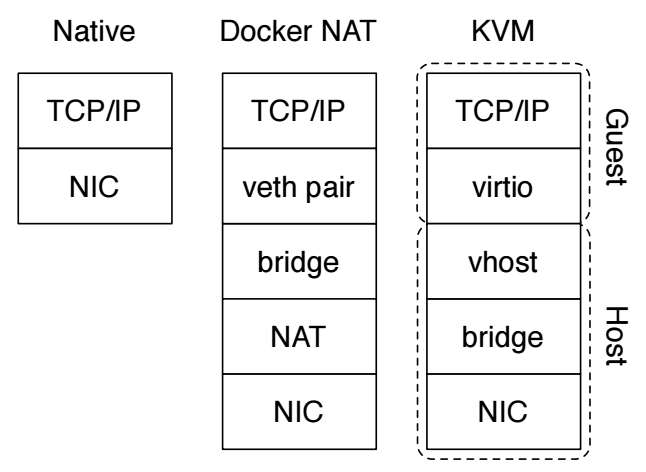
\includegraphics[width=0.5\textwidth]{chapters/measurements/images/network-stack.png}
	\caption[Network stack in different environments]{Network stack in different virtualization
		environments.}
	\label{img:measurements-network-result-stacks}
\end{figure}